\documentclass[
11pt, % The default document font size, options: 10pt, 11pt, 12pt
%codirector, % Uncomment to add a codirector to the title page
]{charter} 


% El títulos de la memoria, se usa en la carátula y se puede usar el cualquier lugar del documento con el comando \ttitle
\titulo{Monitoreo inteligente para plantaciones agrícolas basado en visión por computadora} 

% Nombre del posgrado, se usa en la carátula y se puede usar el cualquier lugar del documento con el comando \degreename
\posgrado{Carrera de Maestría en inteligencia artificial embebida} 
%\posgrado{Carrera de Especialización en Internet de las Cosas} 
%\posgrado{Carrera de Especialización en Inteligencia Artificial}
%\posgrado{Maestría en Sistemas Embebidos} 
%\posgrado{Maestría en Internet de las cosas}
% IMPORTANTE: no omitir titulaciones ni tildación en los nombres, también se recomienda escribir los nombres completos (tal cual los tienen en su documento)
% Tu nombre, se puede usar el cualquier lugar del documento con el comando \authorname
\autor{Esp. Lic. Dante Mendoza}

% El nombre del director y co-director, se puede usar el cualquier lugar del documento con el comando \supname y \cosupname y \pertesupname y \pertecosupname
\director{Lic. Fernando Heredia}
\pertenenciaDirector{UNO} 
\codirector{} % para que aparezca en la portada se debe descomentar la opción codirector en los parámetros de documentclass
\pertenenciaCoDirector{FIUBA}

% Nombre del cliente, quien va a aprobar los resultados del proyecto, se puede usar con el comando \clientename y \empclientename
\cliente{Universidad Nacional del Oeste}
\empresaCliente{UNO}
 
\fechaINICIO{29 de abril de 2025}		%Fecha de inicio de la cursada de GdP \fechaInicioName
\fechaFINALPlan{10 de junio de 2025} 	%Fecha de final de cursada de GdP
\fechaFINALTrabajo{18 de diciembre de 2025}	%Fecha de defensa pública del trabajo final


\begin{document}

\maketitle
\thispagestyle{empty}
\pagebreak


\thispagestyle{empty}
{\setlength{\parskip}{0pt}
\tableofcontents{}
}
\pagebreak


\section*{Registros de cambios}
\label{sec:registro}


\begin{table}[ht]
\label{tab:registro}
\centering
\begin{tabularx}{\linewidth}{@{}|c|X|c|@{}}
\hline
\rowcolor[HTML]{C0C0C0} 
Revisión & \multicolumn{1}{c|}{\cellcolor[HTML]{C0C0C0}Detalles de los cambios realizados} & Fecha      \\ \hline
0      & Creación del documento                                 &\fechaInicioName \\ \hline
1      & Se completa hasta el punto 5 inclusive                & {13} de {mayo} de 2025 \\ \hline
2      & Se completa hasta el punto 9 inclusive
%		  Se puede agregar algo más \newline
%		  En distintas líneas \newline
                                                 & {20} de {mayo} de 2025 \\ \hline
3      & Se completa hasta el punto 12 inclusive                & {27} de {mayo} de 2025 \\ \hline
4      & Se completa el plan	                                 & {03} de {junio} de 2025 \\ \hline

% Si hay más correcciones pasada la versión 4 también se deben especificar acá

\end{tabularx}
\end{table}

\pagebreak



\section*{Acta de constitución del proyecto}
\label{sec:acta}

\begin{flushright}
Buenos Aires, \fechaInicioName
\end{flushright}

\vspace{2cm}

Por medio de la presente se acuerda con el \authorname\hspace{1px} que su Trabajo Final de la \degreename\hspace{1px} se titulará ``\ttitle'' y consistirá en la implementación de un prototipo de un sistema de inspección de plantaciones. El trabajo tendrá un presupuesto preliminar estimado de 725 horas y un costo estimado de \$ 1.082.250 pesos argentinos (ARS), con fecha de inicio el \fechaInicioName\hspace{1px} y fecha de presentación pública en diciembre del 2025.

Se adjunta a esta acta la planificación inicial.

%\fechaFinalName. QUIZAS LUEGO DEBA USUARLO

\vfill

% Esta parte se construye sola con la información que hayan cargado en el preámbulo del documento y no debe modificarla
\begin{table}[ht]
\centering
\begin{tabular}{ccc}
\begin{tabular}[c]{@{}c@{}}Dr. Ing. Ariel Lutenberg \\ Director posgrado FIUBA\end{tabular} & \hspace{2cm} & \begin{tabular}[c]{@{}c@{}}\clientename \\ \empclientename \end{tabular} \vspace{2.5cm} \\ 
\multicolumn{3}{c}{\begin{tabular}[c]{@{}c@{}} \supname \\ Director del Trabajo Final\end{tabular}} \vspace{2.5cm} \\
\end{tabular}
\end{table}




\section{1. Descripción técnica-conceptual del proyecto a realizar}
\label{sec:descripcion}

En la Argentina la actividad relacionada con la cosecha del kiwi ha ganado una relevancia creciente en las últimas décadas, donde maximizar las ganancias es crucial para que sea una actividad redituable. 

Actualmente, el volumen de cosecha se estima mediante el conteo de frutos por unidad de superficie en una etapa avanzada de desarrollo. Sin embargo, esta estimación tardía resulta demasiado cercana al momento de la cosecha y presenta grandes dificultades en plantaciones de tamaño mediano o grande. Una estimación temprana del rendimiento permitiría tomar decisiones tanto operativas como estratégicas. Desde el punto de vista operativo, facilitaría una planificación más racional del uso de los recursos. Desde el punto de vista estratégico, haría posible anticipar la negociación de la producción en los mercados interno o externo.

Por lo tanto, el objetivo de este proyecto es desarrollar un prototipo que permita realizar una estimación temprana del volumen de cosecha de kiwi mediante la captura automatizada de imágenes y el registro de datos ambientales en el terreno. Para ello, el dispositivo estará equipado con cámaras, sensores ultrasónicos, pantalla LCD, lector de tarjetas microSD, y sensores de temperatura y humedad. El dispositivo será montado sobre un medio de transporte adecuado a las características de la plantación. Permitirá la captura automática de imágenes de los frutos, así como el registro de datos ambientales relevantes durante el recorrido. Todos los datos se almacenarán localmente en una tarjeta microSD. Posteriormente, las imágenes serán procesadas mediante técnicas de visión por computadora para detectar objetos relevantes, como frutos en etapas tempranas de maduración. De este modo, se obtendrá una estimación del volumen de cosecha.

Finalmente, la información sobre los frutos detectados y los datos meteorológicos se utilizarán para aplicar técnicas de agrupamiento no supervisado, con el fin de identificar patrones ocultos entre las variables ambientales y la cantidad de frutos, y segmentar automáticamente zonas con comportamientos similares. Toda la información generada se almacenará en un archivo de texto plano. Esta solución proporcionará al productor información valiosa para la toma de decisiones en relación con la planificación y ejecución de la cosecha. En la figura \ref{fig:diagBloques}, se puede apreciar un diagrama de bloques del prototipo.

\begin{figure}[htpb]
\centering 
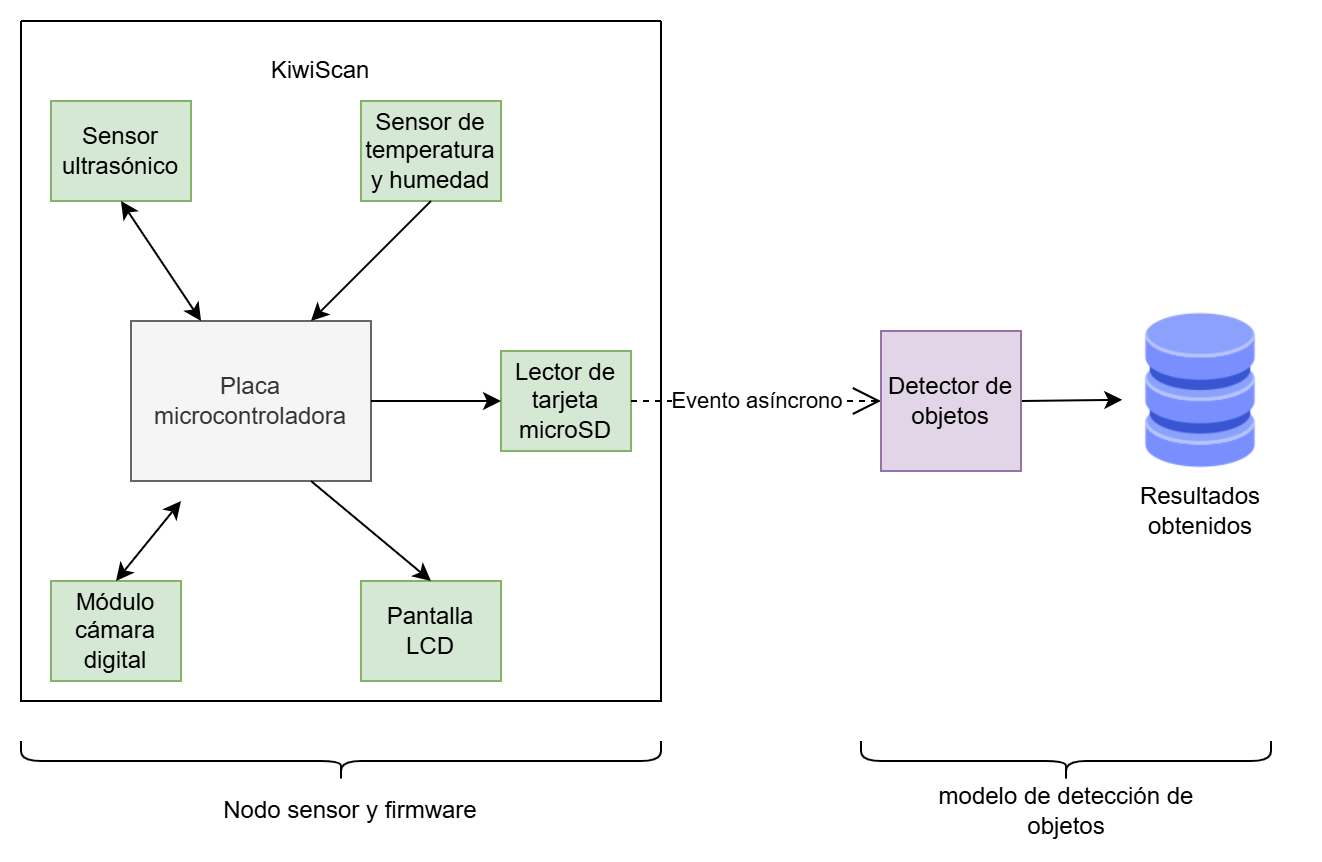
\includegraphics[width=.90\textwidth]{./Figuras/KiwiScan.png}
\caption{Diagrama en bloques del sistema.}
\label{fig:diagBloques}
\end{figure}

\vspace{10px}


\section{2. Identificación y análisis de los interesados}
\label{sec:interesados}

En este apartado, se definirán los involucrados dentro del presente proyecto.

\begin{table}[ht]
%\caption{Identificación de los interesados}
%\label{tab:interesados}
\begin{tabularx}{\linewidth}{@{}|l|X|X|l|@{}}
\hline
\rowcolor[HTML]{C0C0C0} 
Rol           & Nombre y Apellido & Organización 	& Puesto 	\\ \hline
Cliente       & \clientename      &\empclientename	& -       	\\ \hline
Responsable   & \authorname       & FIUBA        	& Alumno 	\\ \hline
Colaboradores & Lic. Aldana Ojeda  & -            & Investigadora       	\\ \hline
Orientador    & \supname	      & \pertesupname 	& Director del Trabajo Final \\ \hline
Usuario final   & Agricultores	      & - 	& - \\ \hline
\end{tabularx}
\end{table}

Por lo tanto, es importante destacar algunas características de los involucrados mencionados:

\begin{itemize}
	\item Orientador: \supname\hspace{1px} es experto en la temática y va a ayudar con la definición de los requerimientos y el desarrollo del modelo de detección de objetos.
	\item Colaboradores: lic. Aldana Ojeda es investigadora ad honorem con experiencia en el área.
    \item Cliente: la universidad UNO es la principal interesada en llevar a cabo este trabajo de investigación.
    \item Usuario final: los agricultores serán los beneficiarios de la implementación.
    \item Responsable: será quien dispondrá del conocimiento y desarrollo del proyecto.
\end{itemize}


\section{3. Propósito del proyecto}
\label{sec:proposito}

La importancia de este proyecto radica en su potencial para automatizar y agilizar el proceso de inspección de plantaciones de kiwis, ofreciendo una alternativa eficiente y tecnológica a los métodos manuales tradicionales. Al integrar dispositivos de captura de imágenes y recolección de datos ambientales con técnicas de visión por computadora y análisis no supervisado, se proporciona una herramienta  que permite estimar con mayor anticipación el volumen de producción. Esto no solo mejora la precisión en la planificación de la cosecha, sino que también optimiza el uso de los recursos disponibles, al generar un impacto positivo en la eficiencia y rentabilidad del productor.

\section{4. Alcance del proyecto}
\label{sec:alcance}

El proyecto incluye:
\begin{itemize}
    \item Desarrollo de un prototipo funcional.
    \item Desarrollo del modelo de detección de objetos.
    \item Toma de imágenes para entrenamiento del modelo.
    \item Clasificación y etiquetado de las imágenes.
    \item Aplicar técnicas de agrupamiento no supervisado (\textit{clustering}).
    \item Pruebas de funcionamiento.
\end{itemize}

El proyecto no incluye:
\begin{itemize}
	
    \item Diseño y fabricación del gabinete que alojará al prototipo.
    \item Manuales de instalación y de usuario del dispositivo.
\end{itemize}


\section{5. Supuestos del proyecto}
\label{sec:supuestos}

Para el desarrollo del presente proyecto, se estima que se dispondrá de los siguientes elementos o consideraciones:

\begin{itemize}
    \item Expertos en la plantación de kiwis, disponibles para consultas.
    \item Servicios en la nube para almacenamiento.
    \item Herramientas de análisis de datos.
    \item Horas hombre para la codificación.
    \item Equipo de trabajo disponible para realizar reuniones.
    \item Equipamiento informático.
    \item Licencias de software.
    \item Artículos de librería.
    \item Embalaje y protección.
    \item Pasajes y viáticos para visita a la plantación.
    \item Presupuesto adicional para imprevistos.
    \item La previsión de costos no superará en gran medida lo estimado.
\end{itemize}


\section{6. Requerimientos}
\label{sec:requerimientos}
Esta sección detalla los requerimientos del software, delineando las funcionalidades y características necesarias para cumplir con los objetivos del proyecto.

\begin{enumerate}
	\item Requerimientos funcionales:
		\begin{enumerate}
			\item El sistema debe registrar la temperatura del ambiente.
			\item El sistema debe registrar la humedad del ambiente.
			\item El sistema debe informar el espacio disponible de la tarjeta microSD.
            \item El sistema debe informar la cantidad de fotos tomadas.
            \item El sistema debe contabilizar los frutos detectados en cada imagen.
            \item El sistema debe informar el volumen total estimado de cosecha.
            \item Generar un resumen final con la segmentación de zonas que presentaron comportamientos similares en la producción.
		\end{enumerate}
	\item Requerimientos no funcionales:
		\begin{enumerate}
			\item El sistema debe ser escalable, de forma de poder agregar más sensores en el futuro.
			\item El firmware debe estar modularizado.
            \item El firmware debe estar sobre un sistema operativo.
            \item El modelo de IA debe ser capaz de identificar frutos en diferentes estados de maduración con al menos un 80\% de precisión en condiciones normales de luz.
            \item El modelo de detección debe ejecutarse de forma local o en un entorno que no dependa de conectividad a internet.
            \item El sistema debe aplicar algoritmos de agrupamiento no supervisado (por ejemplo, K-means o DBSCAN) para segmentar zonas de producción según las variables registradas.
		\end{enumerate}
    \item Requerimientos de interfaz gráfica en la pantalla LCD:
		\begin{enumerate}
			\item Se debe mostrar los valores de humedad y temperatura.
			\item Se debe mostrar el espacio disponible en la tarjeta microSD.
            \item Se debe mostrar la cantidad de fotos tomadas.
            \item La información en pantalla debe actualizarse cada 5 segundos.
		\end{enumerate}
        \newpage
    \item Requerimientos de interoperabilidad:
		\begin{enumerate}
			\item Las fotos deben almacenarse en un formato de archivo JPG o JPEG.
			\item Las imágenes capturadas deben tener un mínimo de resolución de 640 x 480.
            \item Cada imagen guardada no debe superar los 10 MB.
		\end{enumerate}
    \item Requerimientos de documentación:
		\begin{enumerate}
			\item Se debe presentar un informe de avance del proyecto.
			\item Se debe presentar una memoria técnica al final del proyecto.
		\end{enumerate}
\end{enumerate}


\section{7. Historias de usuarios (\textit{Product backlog})}
\label{sec:backlog}

Se utiliza la serie de Fibonacci: 0, 1, 3, 5, 8, 13, 21, 34. . . para establecer los pesos de las historias de usuario. Se suman los pesos de: cantidad de esfuerzo a realizar, complejidad del trabajo y riesgo o incertidumbre del proyecto. Si el peso no coincide con alguno de la serie se asigna el inmediato superior.

Tabla de pesos:
\begin{enumerate}
\item Cantidad de trabajo a realizar
	\begin{enumerate}
	\item Bajo $\rightarrow$ peso 1 
	\item Medio $\rightarrow$ peso 3
	\item Alto $\rightarrow$ peso 5
	\end{enumerate}
\item Complejidad del trabajo a realizar
	\begin{enumerate}
	\item Bajo $\rightarrow$ peso 1 
	\item Medio $\rightarrow$ peso 3
	\item Alto $\rightarrow$ peso 5
	\end{enumerate}
\item Riesgo o incertidumbre del trabajo a realizar
	\begin{enumerate}
	\item Bajo $\rightarrow$ peso 1 
	\item Medio $\rightarrow$ peso 3
	\item Alto $\rightarrow$ peso 5
	\end{enumerate}
\end{enumerate}

Historia de usuario 1: “Como agricultor quiero ver la cantidad de frutos estimados para planificar la cosecha."
\\
Dificultad: alto (5) $\rightarrow$ Porque involucra muchas horas de ingeniería y desarrollo.
\\
Complejidad: medio (3) $\rightarrow$ Hay que obtener las imágenes de la plantación.
\\
Riesgo: medio (3) $\rightarrow$ Problemas que un evento climático arruine la cosecha y por ende la fuente de datos a utilizar.
\\
Story Point = 13
\\
\\
Historia de usuario 2: “Como agricultor quiero ver la temperatura del día en que se tomaron las fotos para comprobar si es adecuado para el tipo de fruto."
\\
Dificultad: bajo (1) $\rightarrow$ Por que no involucra muchas horas de ingeniería y desarrollo.
\\
Complejidad: bajo (1) $\rightarrow$ El módulo DHT11 es sencillo de utilizar.
\\
Riesgo: bajo (1) $\rightarrow$ El módulo DHT11 tiene una precisión que ronda los +-2 del valor real.
\\
Story Point = 3
\\
\\
Historia de usuario 3: “Como agricultor quiero ver la humedad del día en que se tomaron las fotos para comprobar si es adecuado para el tipo de fruto."
\\
Dificultad: bajo (1) $\rightarrow$ Por que no involucra muchas horas de ingeniería y desarrollo.
\\
Complejidad: bajo (1) $\rightarrow$ El módulo DHT11 es sencillo de utilizar.
\\
Riesgo: bajo (1) $\rightarrow$ El módulo DHT11 tiene una precisión que ronda los +-2 del valor real.
\\
Story Point = 3
\\
\\
Historia de usuario 4: “Como operario quiero ver la cantidad de memoria disponible en la tarjeta microSD para comprobar si puedo continuar con la actividad."
\\
Dificultad: medio (3) $\rightarrow$ Por que involucra muchas horas de ingeniería y desarrollo.
\\
Complejidad: medio (3) $\rightarrow$ Se conoce que trabajar con tarjetas microSD tiene cierta complejidad.
\\
Riesgo: medio (3) $\rightarrow$ Que tal vez no se puedan reconocer tarjetas microSD de determinados fabricantes.
\\
Story Point = 13
\\
\\
Historia de usuario 5: “Como operario quiero ver la cantidad de fotos que fueron tomadas durante el recorrido para comprobar si el proceso funcionó correctamente."
\\
Dificultad: medio (3) $\rightarrow$ Por que involucra muchas horas de ingeniería y desarrollo.
\\
Complejidad: medio (3) $\rightarrow$ Se conoce que trabajar con tarjetas microSD tiene cierta complejidad.
\\
Riesgo: medio (3) $\rightarrow$ Que tal vez no se puedan reconocer tarjetas microSD de determinados fabricantes.
\\
Story Point = 13
\\
\\
Historia de usuario 6: “Como agricultor deseo ver cuántos frutos fueron detectados en cada imagen para ver el estado de maduración"
\\
Dificultad: medio (3) $\rightarrow$ Por que involucra muchas horas de ingeniería y desarrollo.
\\
Complejidad: medio (3) $\rightarrow$ Se conoce que trabajar con modelos de detección de objetos tiene determinada complejidad.
\\
Riesgo: medio (3) $\rightarrow$ Que tal vez no se logren detectar todos los frutos presente en la imagen.
\\
Story Point = 13
\\
\\
Historia de usuario 7: “Como agricultor deseo ver el volumen total de cosecha estimado para decidir su recolección."
\\
Dificultad: medio (3) $\rightarrow$ Por que involucra muchas horas de ingeniería y desarrollo.
\\
Complejidad: medio (3) $\rightarrow$ Se conoce que trabajar con modelos de detección de objetos tiene determinada complejidad.
\\
Riesgo: medio (3) $\rightarrow$ Que tal vez no se logren detectar todos los frutos presente en todas las imágenes.
\\
Story Point = 13
\\
\\
Historia de usuario 8: “Como agricultor deseo ver si existe alguna relación entre la producción y los datos ambientales para encontrar zonas más beneficiosas en la plantación."
\\
Dificultad: medio (3) $\rightarrow$ Por que involucra muchas horas de ingeniería y desarrollo.
\\
Complejidad: medio (3) $\rightarrow$ Se conoce que trabajar con técnicas de agrupamiento es complejo.
\\
Riesgo: medio (3) $\rightarrow$ Que tal vez no se logre encontrar ninguna agrupación con los datos recolectados.
\\
Story Point = 13
\\
\\
Historia de usuario 9: “Como agricultor deseo que el sistema genere un resumen de toda la información procesada para tomar decisiones logísticas."
\\
Dificultad: bajo (1) $\rightarrow$ Por que no tiene mayor dificultad resumir toda la información generada.
\\
Complejidad: bajo (1) $\rightarrow$ Su desarrollo no sería complejo.
\\
Riesgo: bajo (1) $\rightarrow$ Que tal vez no haya información de entrada suficiente como para generar un resumen.
\\
Story Point = 3


\section{8. Entregables principales del proyecto}
\label{sec:entregables}

Los entregables del proyecto son:

\begin{itemize}
	\item Código fuente no editable.
        \item Conjunto de imágenes etiquetadas para entrenamiento del modelo.
        \item Modelo entrenado para detectar los frutos de la plantación.
	\item Diagrama de instalación.
	\item Documentación del proyecto.
\end{itemize}


\section{9. Desglose del trabajo en tareas}
\label{sec:wbs}

\begin{enumerate}
\item Documentación y análisis preliminar (75 h)
	\begin{enumerate}
	\item Planificación del proyecto (20 h)
	\item Especificación de requisitos de software (40 h)
	\item Definición de las pruebas de aceptación (15 h)
	\end{enumerate}
\item Búsqueda de material bibliográfico (100 h)
	\begin{enumerate}
	\item Buscar hojas de datos de todos los componentes (40 h)
	\item Buscar modelos de visión por computadora (40 h)
	\item Investigar sobre dispositivos con funciones similares (20 h)
	\end{enumerate}
\item Comprensión del objeto de trabajo (90 h)
	\begin{enumerate}
	\item Estudiar cómo se compone una plantación de kiwi (20 h)
	\item Características y tipos de frutos (20 h)
	\item Métodos de estimación de la cosecha (20 h)
	\item Impacto de las variables climatológicas (20 h)
	\item Reuniones con especialistas en la plantación (10 h)
	\end{enumerate}
 \item Preparación del hardware y modelo (80 h)
	\begin{enumerate}
	\item Selección de componentes (30 h)
	\item Configuraciones de los componentes (30 h)
	\item Pruebas de funcionamiento (20 h)
	\end{enumerate}
 \item Desarrollo del firmware y modelo (230 h)
	\begin{enumerate}
	\item Diseño de la arquitectura del firmware (20 h)
	\item Desarrollo de los drivers del dispositivo (60 h)
	\item Montar el sistema operativo (15 h)
	\item Implementar la biblioteca HAL (10 h)
	\item Integración de los módulos (35 h)
    \item Recolección de imágenes para entrenamiento (30 h)
	\item Selección y etiquetado de imágenes (15 h)
    \item Desarrollo y configuración del modelo (10 h)
	\item Entrenamiento del modelo (35 h)
	\end{enumerate}
 \item Testing (30 h)
	\begin{enumerate}
	\item Testeo del firmware (10 h)
	\item Testeo del modelo (10 h)
	\item Depuración general (10 h)
	\end{enumerate}
 \item Cierre del proyecto (120 h)
	\begin{enumerate}
	\item Informes de avance del proyecto (20 h)
	\item Elaboración de la memoria técnica del trabajo final (80 h)
	\item Presentación final del proyecto (20 h)
	\end{enumerate}
\end{enumerate}

Cantidad total de horas: (725 h)

\begin{landscape}
\section{10. Diagrama de Activity On Node}
\label{sec:AoN}

En la figura \ref{fig:DAON} se resalta en color rojo las flechas que corresponden al camino crítico y a las que hay que prestar mayor atención. La suma del camino crítico estima un tiempo de desarrollo del proyecto de 580 horas.

\begin{figure}[htpb]
\centering 
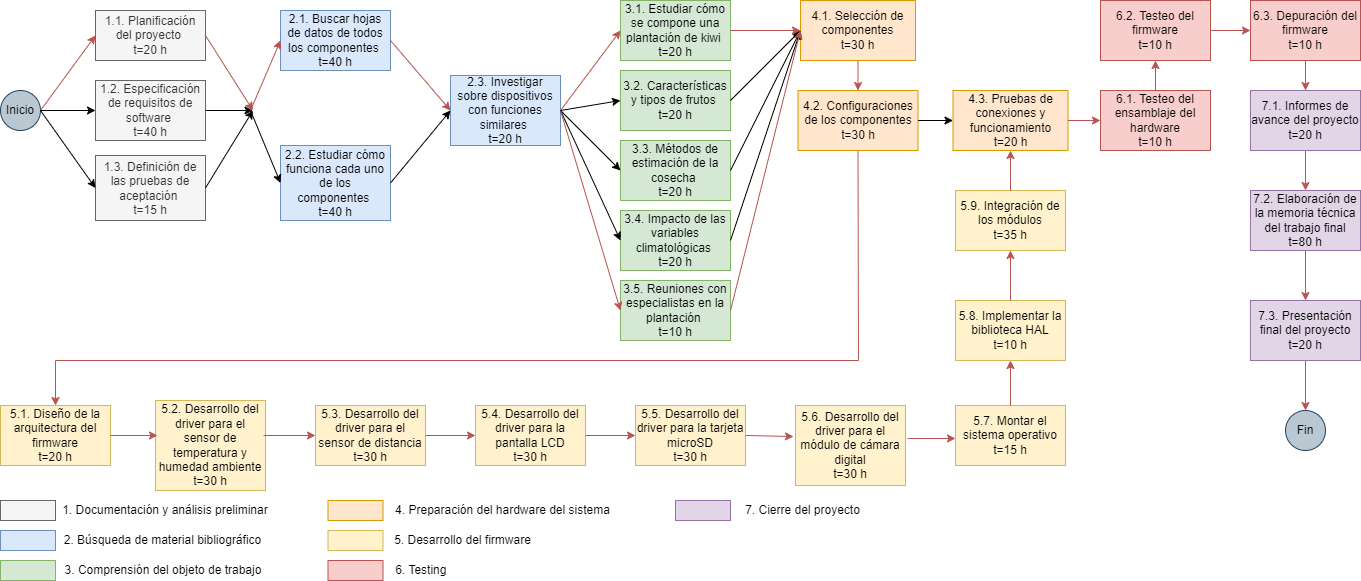
\includegraphics[width=24cm , height=11cm]{./Figuras/DAON.png}
\caption{Diagrama de \textit{Activity on Node}.}
\label{fig:DAON}
\end{figure}

\end{landscape}


\section{11. Diagrama de Gantt}
\label{sec:gantt}

En la figura \ref{fig:gantt} se muestra el diagrama de Gantt del proyecto. Para su realización se estableció un horario laboral de 4 horas de lunes a viernes.

\begin{figure}[htpb]
  \begin{center}
    \begin{ganttchart}[
      time slot unit=day,
      time slot format=isodate,
      x unit=0.038cm,
      y unit title=0.4cm,
      y unit chart=0.6cm,
      milestone/.append style={xscale=4}
      ]{2025-06-02}{2025-12-15}
      
      \gantttitlecalendar*{2025-06-02}{2025-12-15}{year} \\
      \gantttitlecalendar*{2025-06-02}{2025-12-15}{month} \\
      
      \ganttgroup{Duración Total}{2025-06-02}{2025-12-15} \\
      
      %%%%%%%%%%%%%%%%% 1. Documentación y análisis preliminar
      \ganttgroup{1. Documentación y análisis preliminar}{2025-06-02}{2025-06-09} \\
      \ganttbar{1.1 Planificación del proyecto}{2025-06-02}{2025-06-04} \\
      \ganttbar{1.2 Especificación de requisitos de software}{2025-06-05}{2025-06-07} \\
      \ganttbar{1.3 Definición de pruebas de aceptación}{2025-06-08}{2025-06-09} \\
      
      %%%%%%%%%%%%%%%%% 2. Búsqueda de material bibliográfico
      \ganttgroup{2. Búsqueda de material bibliográfico}{2025-06-10}{2025-06-23} \\
      \ganttbar{2.1 Buscar hojas de datos de componentes}{2025-06-10}{2025-06-15} \\
      \ganttbar{2.2 Buscar modelos de visión por computadora}{2025-06-16}{2025-06-20} \\
      \ganttbar{2.3 Investigar dispositivos similares}{2025-06-21}{2025-06-23} \\
      
      %%%%%%%%%%%%%%%%% 3. Comprensión del objeto de trabajo
      \ganttgroup{3. Comprensión del objeto de trabajo}{2025-06-24}{2025-07-11} \\
      \ganttbar{3.1 Composición de plantaciones de kiwi}{2025-06-24}{2025-06-27} \\
      \ganttbar{3.2 Características y tipos de frutos}{2025-06-30}{2025-07-03} \\
      \ganttbar{3.3 Estimación de la cosecha}{2025-07-04}{2025-07-07} \\
      \ganttbar{3.4 Variables climatológicas}{2025-07-08}{2025-07-10} \\
      \ganttbar{3.5 Reuniones con especialistas}{2025-07-11}{2025-07-11} \\
      
      %%%%%%%%%%%%%%%%% 4. Preparación del hardware y modelo
      \ganttgroup{4. Preparación del hardware y modelo}{2025-07-14}{2025-07-28} \\
      \ganttbar{4.1 Selección de componentes}{2025-07-14}{2025-07-18} \\
      \ganttbar{4.2 Configuración de componentes}{2025-07-21}{2025-07-25} \\
      \ganttbar{4.3 Pruebas de funcionamiento}{2025-07-28}{2025-07-28} \\
      
      %%%%%%%%%%%%%%%%% 5. Desarrollo del firmware y modelo
      \ganttgroup{5. Desarrollo del firmware y modelo}{2025-07-29}{2025-09-26} \\
      \ganttbar{5.1 Arquitectura del firmware}{2025-07-29}{2025-07-31} \\
      \ganttbar{5.2 Drivers del dispositivo}{2025-08-01}{2025-08-20} \\
      \ganttbar{5.3 Montar sistema operativo}{2025-08-21}{2025-08-22} \\
      \ganttbar{5.4 Biblioteca HAL}{2025-08-25}{2025-08-26} \\
      \ganttbar{5.5 Integración de módulos}{2025-08-27}{2025-09-01} \\
      \ganttbar{5.6 Recolección de imágenes}{2025-09-02}{2025-09-05} \\
      \ganttbar{5.7 Selección y etiquetado de imágenes}{2025-09-08}{2025-09-10} \\
      \ganttbar{5.8 Desarrollo y configuración del modelo}{2025-09-11}{2025-09-12} \\
      \ganttbar{5.9 Entrenamiento del modelo}{2025-09-15}{2025-09-26} \\
      
      %%%%%%%%%%%%%%%%% 6. Testing
      \ganttgroup{6. Testing}{2025-09-29}{2025-10-03} \\
      \ganttbar{6.1 Testeo del firmware}{2025-09-29}{2025-09-30} \\
      \ganttbar{6.2 Testeo del modelo}{2025-10-01}{2025-10-02} \\
      \ganttbar{6.3 Depuración general}{2025-10-03}{2025-10-03} \\
      
      %%%%%%%%%%%%%%%%% 7. Cierre del proyecto
      \ganttgroup{7. Cierre del proyecto}{2025-10-06}{2025-12-15} \\
      \ganttbar{7.1 Informes de avance del proyecto}{2025-10-06}{2025-10-10} \\
      \ganttbar{7.2 Elaboración de la memoria técnica}{2025-10-13}{2025-12-05} \\
      \ganttbar{7.3 Presentación final del proyecto}{2025-12-08}{2025-12-15} \\
      
    \end{ganttchart}
  \end{center}
  \caption{Diagrama de Gantt del proyecto.}
  \label{fig:gantt}
\end{figure}

%%%%%%%%%%%%%%%%%%%%%%%%%%%%%%


\section{12. Presupuesto detallado del proyecto}
\label{sec:presupuesto}

Los precios expresados en la siguiente tabla se encuentran en peso argentino (ARS) y fue estimado el 13 de mayo del 2025.

\begin{table}[htpb]
\centering
\begin{tabularx}{\linewidth}{@{}|X|c|r|r|@{}}
\hline
\rowcolor[HTML]{C0C0C0} 
\multicolumn{4}{|c|}{\cellcolor[HTML]{C0C0C0}COSTOS DIRECTOS} \\ \hline
\rowcolor[HTML]{C0C0C0} 
Descripción &
  \multicolumn{1}{c|}{\cellcolor[HTML]{C0C0C0}Cantidad} &
  \multicolumn{1}{c|}{\cellcolor[HTML]{C0C0C0}Valor unitario} &
  \multicolumn{1}{c|}{\cellcolor[HTML]{C0C0C0}Valor total} 
  \\ 
  \hline Tarjeta de desarrollo STM32F429ZI
 &
  \multicolumn{1}{c|}{1} &
  \multicolumn{1}{c|}{80 000} &
  \multicolumn{1}{c|}{80 000} 
  \\ 
  \hline Módulo Dht11 Sensor De Temperatura Humedad
 &
  \multicolumn{1}{c|}{1} &
  \multicolumn{1}{c|}{5 000} &
  \multicolumn{1}{c|}{5 000} 
  \\ 
  \hline Sensor Ultrasonico Hc Sr04
 &
  \multicolumn{1}{c|}{1} &
  \multicolumn{1}{c|}{5 000} &
  \multicolumn{1}{c|}{5 000}
  \\ 
  \hline Modulo Display Lcd 16x2 Con I2c
 &
  \multicolumn{1}{c|}{1} &
  \multicolumn{1}{c|}{12 000} &
  \multicolumn{1}{c|}{12 000}
  \\ 
  \hline Módulo Lector De Tarjetas Micro Sd
 &
  \multicolumn{1}{c|}{1} &
  \multicolumn{1}{c|}{8 500} &
  \multicolumn{1}{c|}{8 500}
  \\ 
  \hline Módulo cámara OV7670
 &
  \multicolumn{1}{c|}{1} &
  \multicolumn{1}{c|}{18 000} &
  \multicolumn{1}{c|}{18 000}
  \\ 
  \hline Kit 40 Cables Dupont
 &
  \multicolumn{1}{c|}{1} &
  \multicolumn{1}{c|}{6 000} &
  \multicolumn{1}{c|}{6 000}
  \\ 
  \hline Batería 3.7v 2000 mA
 &
  \multicolumn{1}{c|}{1} &
  \multicolumn{1}{c|}{35 000} &
  \multicolumn{1}{c|}{35 000}
  \\ 
  \hline Cable USB mallado
 &
  \multicolumn{1}{c|}{1} &
  \multicolumn{1}{c|}{10 500} &
  \multicolumn{1}{c|}{10 500}
  \\ 
  \hline Artículos de librería
 &
  \multicolumn{1}{c|}{1} &
  \multicolumn{1}{c|}{30 000} &
  \multicolumn{1}{c|}{30 000}
  \\ 
  \hline Licencias de software
 &
  \multicolumn{1}{c|}{3} &
  \multicolumn{1}{c|}{60 000} &
  \multicolumn{1}{c|}{180 000}
  \\ 
  \hline Servicios en la nube
 &
  \multicolumn{1}{c|}{5} &
  \multicolumn{1}{c|}{45 000} &
  \multicolumn{1}{c|}{225 000}
  \\ 
  \hline Horas de ingeniería
 &
  \multicolumn{1}{c|}{725} &
  \multicolumn{1}{c|}{300} &
  \multicolumn{1}{c|}{217 500}
  \\ 
  \hline
\multicolumn{3}{|c|}{SUBTOTAL} &
  \multicolumn{1}{c|}{832 500} \\ \hline
\rowcolor[HTML]{C0C0C0} 
\multicolumn{4}{|c|}{\cellcolor[HTML]{C0C0C0}COSTOS INDIRECTOS} \\ \hline
\rowcolor[HTML]{C0C0C0} 
Descripción &
  \multicolumn{1}{c|}{\cellcolor[HTML]{C0C0C0}Cantidad} &
  \multicolumn{1}{c|}{\cellcolor[HTML]{C0C0C0}Valor unitario} &
  \multicolumn{1}{c|}{\cellcolor[HTML]{C0C0C0}Valor total} 
  \\ 
  \hline 30 \% de los costos directos
&
\multicolumn{1}{|l|}{1} &
\multicolumn{1}{|l|}{1} &
\multicolumn{1}{|l|}{249 750} 
   \\ \hline
\multicolumn{3}{|c|}{SUBTOTAL} &
  \multicolumn{1}{c|}{249 750} \\ \hline
\rowcolor[HTML]{C0C0C0}
\multicolumn{3}{|c|}{TOTAL} &
\multicolumn{1}{|l|}{1 082 250} 
   \\ \hline 
\end{tabularx}
\end{table}


\section{13. Gestión de riesgos}
\label{sec:riesgos}
En este apartado se mencionan los posibles riesgos del proyecto y el plan de mitigación.

a) Identificación de los riesgos y estimación de sus consecuencias:
 
Riesgo 1: demora para conseguir los componentes electrónicos requeridos.
\begin{itemize}
	\item Severidad (7): el proyecto sufrirá retrasos en su desarrollo.\\
	\item Probabilidad de ocurrencia (6): el mercado local no cuenta con el stock de los componentes necesarios para el proyecto.
\\
\end{itemize}   

Riesgo 2: daño o pérdida del hardware del proyecto.
\begin{itemize}
	\item Severidad (8): esto genera un retraso importante en la ejecución de las actividades del proyecto en la fase de implementación y pruebas.\\
	\item Ocurrencia (4): el encargado del proyecto será una persona muy cuidadosa y responsable.\\
\end{itemize}

Riesgo 3: mala estimación de la planificación.
\begin{itemize}
	\item Severidad (7): el proyecto sufrirá varios cambios y retrasos en la ejecución.\\
	\item Ocurrencia (8): no se cuenta con experiencia en planificación de proyectos.\\
\end{itemize}

Riesgo 4: variación de precios en la compra del hardware y software.
\begin{itemize}
	\item Severidad (8): el capital necesario para adquirir el equipo del proyecto se vería afectado.\\
	\item Ocurrencia (8): se tiene conocimiento de que existe mucha fluctuación en los precios de mercado.\\
\end{itemize}

Riesgo 5: retraso en el desarrollo del firmware y modelo.
\begin{itemize}
	\item Severidad (8): retrasos en el proyecto debido a que el firmware y el modelo es una parte fundamental en la integración e implementación del prototipo.\\
	\item Ocurrencia (7): falta de conocimiento y experiencia en la tecnología trabajada.\\
\end{itemize}

b) Tabla de gestión de riesgos:

\begin{table}[htpb]
\centering
\begin{tabularx}{\linewidth}{@{}|X|c|c|c|c|c|c|@{}}
\hline
\rowcolor[HTML]{C0C0C0} 
Riesgo & S & O & RPN & S* & O* & RPN* \\ \hline
Demora para conseguir los componentes electrónicos requeridos & 7 & 6 & 42  &    &    &      \\ \hline
Daño o pérdida del hardware del proyecto & 8 & 4 & 32  &    &    &      \\ \hline
Mala estimación de la planificación & 7 & 8 & \cellcolor{red}{56}  & 8  & 5  & \cellcolor{green}{40}   \\ \hline
Variación de precios en la compra del hardware y software & 8 & 8 & \cellcolor{red}{64}  & 9 & 5  & \cellcolor{green}{45}   \\ \hline
Retraso en la programación del firmware y modelo & 8 & 7 & \cellcolor{red}{56}  & 8  & 5  & \cellcolor{green}{40}   \\ \hline
\end{tabularx}%
\end{table}

Criterio adoptado: se tomarán medidas de mitigación en los riesgos cuyos números de RPN sean mayores a 45.

Nota: los valores marcados con (*) en la tabla corresponden luego de haber aplicado la mitigación.

c) Plan de mitigación de los riesgos que originalmente excedían el RPN máximo establecido:
 
Riesgo 3*: se consultará con el director la planificación para ajustar los tiempos de las tareas de acuerdo a su experiencia.
  \begin{itemize}
	\item Severidad (8): probabilidad que se modifiquen tiempos ya definidos a tareas.
	\item Probabilidad de ocurrencia (5): Se reduce el riesgo de hacer una mala planificación del proyecto.
	\end{itemize}

Riesgo 4*: se consultará con el cliente la posibilidad de efectuar compras de hardware y software con anticipación.
  \begin{itemize}
	\item Severidad (9): puede que el cliente no disponga de capital para hacer una compra anticipada.
	\item Probabilidad de ocurrencia (5): se reduce el riesgo de variación de precios.
	\end{itemize}

Riesgo 5*: Se dedicará más tiempo a la investigación de la tecnología y se buscará ayuda en algún ingeniero que haya desarrollado proyectos de estas características.
  \begin{itemize}
	\item Severidad (8): No cambia.
	\item Probabilidad de ocurrencia (5): Se obtendrá mayor conocimiento y experiencia en este tipo de tecnología.
	\end{itemize}


\section{14. Gestión de la calidad}
\label{sec:calidad}

Para cada uno de los requerimientos funcionales, a continuación, se lista su respectiva verificación y validación. Estas serán llevadas a cabo por el responsable del proyecto.

\begin{itemize} 
\item Req \#1.1: El sistema debe registrar la temperatura del ambiente.
\begin{itemize}
	\item Verificación: Revisar que el módulo realiza la toma de temperatura correctamente.
	\item Validación: Probar que se obtuvieron los valores del sensor mostrando los datos obtenidos en un monitor serial.
\end{itemize}
\end{itemize}

\begin{itemize} 
\item Req \#1.2: El sistema debe registrar la humedad del ambiente.
\begin{itemize}
	\item Verificación: Revisar que el módulo realiza la toma de humedad correctamente.
	\item Validación: Probar que se obtuvieron los valores del sensor mostrando los datos obtenidos en un monitor serial.
\end{itemize}
\end{itemize}

\begin{itemize} 
\item Req \#1.3: El sistema debe informar el espacio disponible de la tarjeta microSD.
\begin{itemize}
	\item Verificación: Revisar que el módulo realiza el registro de la información guardada.
	\item Validación: Conectar la tarjeta microSD en una computadora para comparar el espacio disponible con lo informado por el sistema.
\end{itemize}
\end{itemize}

\begin{itemize} 
\item Req \#1.4: El sistema debe informar la cantidad de fotos tomadas.
\begin{itemize}
	\item Verificación: Revisar si se guardan las fotografías en el medio de almacenamiento.
	\item Validación: Probar de contabilizar el total de fotos y mostrar el valor en un monitor serial.
\end{itemize}
\end{itemize}

\begin{itemize} 
\item Req \#1.5: El sistema debe contabilizar los frutos detectados en cada imagen.
\begin{itemize}
	\item Verificación: Revisar si las salidas contienen frutos detectados en la imagen.
	\item Validación: Probar de contabilizar el total de elementos manualmente y compararlo con la salida generada.
\end{itemize}
\end{itemize}

\begin{itemize} 
\item Req \#1.6: El sistema debe informar el volumen total estimado de cosecha.
\begin{itemize}
	\item Verificación: Revisar la sumatoria final obtenida.
	\item Validación: Probar de contabilizar el total de frutos en cada imagen y compararlo con el resultado final generado.
\end{itemize}
\end{itemize}

\begin{itemize} 
\item Req \#1.7: Generar un resumen final con la segmentación de zonas que presentaron comportamientos similares en la producción.
\begin{itemize}
	\item Verificación: Revisar si el informe generado es correcto en su estructura.
	\item Validación: Ver si las zonas indicadas efectivamente tienen relación en la producción.
\end{itemize}
\end{itemize}

\begin{itemize} 
\item Req \#2.2: El firmware debe estar modularizado.
\begin{itemize}
	\item Verificación: Comprobar si se armaron distintos módulos para cada dispositivo.
	\item Validación: Hacer funcionar cada módulo de manera aislada para ver los resultados obtenidos.
\end{itemize}
\end{itemize}

\begin{itemize} 
\item Req \#2.3: El firmware debe estar sobre un sistema operativo.
\begin{itemize}
	\item Verificación: Revisar el funcionamiento del sistema operativo.
	\item Validación: Realizar llamadas al sistema operativo y comprobar su respuesta.
\end{itemize}
\end{itemize}

\begin{itemize} 
\item Req \#3.4: La información en pantalla debe actualizarse cada 5 segundos.
\begin{itemize}
	\item Verificación: Revisar el funcionamiento de la pantalla LCD.
	\item Validación: Inspeccionar visualmente si la información mostrada es actualizada en el lapso de tiempo establecido.
\end{itemize}
\end{itemize}

\begin{itemize} 
\item Req \#4.1: Las fotos deben almacenarse en un formato de archivo JPG o JPEG.
\begin{itemize}
	\item Verificación: Revisar si la imagen está almacenada correctamente.
	\item Validación: Inspeccionar visualmente en una computadora si la imagen tiene la extensión de archivo esperada.
\end{itemize}
\end{itemize}

\begin{itemize} 
\item Req \#4.2: Las imágenes capturadas deben tener un mínimo de resolución de 640 x 480.
\begin{itemize}
	\item Verificación: Revisar si la imagen está almacenada correctamente.
	\item Validación: Inspeccionar visualmente en una computadora si la resolución de archivo es la esperada.
\end{itemize}
\end{itemize}

\begin{itemize} 
\item Req \#4.3: Cada imagen guardada no debe superar los 10 MB.
\begin{itemize}
	\item Verificación: Revisar si la imagen está almacenada correctamente.
	\item Validación: Inspeccionar visualmente en una computadora si el tamaño de archivo es el esperado.
\end{itemize}
\end{itemize}

\begin{itemize} 
\item Req \#5.2: Se debe presentar una memoria técnica al final del proyecto.
\begin{itemize}
	\item Verificación: Verificar que se haya presentado la memoria técnica del proyecto.
	\item Validación: Revisar que se cumplieron los requerimientos estipulados en el plan de proyecto.
\end{itemize}
\end{itemize}


\section{15. Procesos de cierre}    
\label{sec:cierre}
En esta sección se establecen las pautas de trabajo para realizar una reunión final de evaluación del proyecto, tal que contemple las siguientes actividades:

\begin{itemize}
	\item Pautas de trabajo que se seguirán para analizar si se respetó el Plan de Proyecto original:\\
    \begin{itemize}
        \item Encargado: \authorname
        \item Procedimiento: Se analizará el cumplimiento con los requerimientos y cronograma establecidos. En el caso de hallar requerimientos incumplidos y/o retrasos en las tareas se evaluarán las causas y se propondrán acciones para evitarlo en futuros proyectos.
    \end{itemize}
\end{itemize}

\begin{itemize}
	\item Identificación de las técnicas y procedimientos útiles e inútiles que se emplearon, y los problemas que surgieron y cómo se solucionaron:\\
    \begin{itemize}
        \item Encargado: \authorname
        \item Procedimiento: Se evaluarán los procedimientos utilizados en función a su utilidad y eficiencia para alcanzar los objetivos predefinidos. Se analizarán los problemas surgidos y las medidas paliativas.
    \end{itemize}
\end{itemize}

\begin{itemize}
	\item Indicar quién organizará el acto de agradecimiento a todos los interesados, y en especial al equipo de trabajo y colaboradores:\\
    \begin{itemize}
        \item Encargado: \authorname
        \item Procedimiento: Tras la exposición pública del proyecto frente al jurado, se llevará a cabo un expresivo reconocimiento hacia aquellos que contribuyeron a su realización, incluyendo al director del trabajo, los miembros del jurado y las autoridades de la MIAE.
    \end{itemize}
\end{itemize}


\end{document}